\documentclass[12pt]{article}
\usepackage{graphicx}
\graphicspath{ {./images/} }
\usepackage[utf8]{inputenc}
\begin{document}
\begin{figure}[t]

\includegraphics[height=6cm]{rut}
\centering
\end{figure}
\title{\textbf{Intro to Artificial Intelligence \\ Project 2}}
\author{-- Maxwell Legrand -- \\
-- Arbazkhan Pathan -- \\
-- Tarek Mohammed --
}
\date{August 2020}



\maketitle

\pagebreak

\section{Implementation}

\subsection{Naive Bayes}

\subsubsection{Digit}
\paragraph{In order to implement Naive Bayes Digit Classification we took the following steps:}
\begin{itemize}
    \item[1.] Load Data
    \item[] Digit Images have a height of 28 characters and a width of 28 characters. By storing each image as an array inside of an encapsulating array that contains all the images we are able to shuffle the trianing data to ensure there is no bias that occurs. In order to make the image data usable, each character ("pixel") is converted from a text equivalent to an integer value; ' ' being equivalent to 0, '\#' being equivalent to 1, and '+' being equivalent to 2.
    \item[2.] Training 
    \item[] Before the training step, the selected data is randomized to prevent training bais from occurring. For each image in the training set, the occurence of each digit in the labels is recorded and used to calculate the prior probability for each digit. This is done by taking the occurence for each digit and dividing by the training size. This gives us the following formula:
    \item[] $\hat{P}(x) = \frac{o(x)}{n}$ , where $\hat{P}(x)$ represents the previous probability of a digit, $x$; $o(x)$ represents the count of occurences for that digit; and $n$ is the total size of the training data
    \item[3.] Pixel Probablilities
    \item[] A "feature" array for each image is generated based on the height and width of the image. For each instance of a pixel that is not blank, a '1' is added into the feature array (and a '0' if the pixel is blank). The probablity of each pixel in each digit is calculated by taking the occurences of each pixel divided by total pixel count: $\hat{P}(p|x) = \frac{o(p, x)}{n}$ where $\hat{P}(p|x)$ is the probabliity of a pixel, $p$, given the digit, $x$; $o(p, x)$ is the occurences of the specific pixel in the digit; $n$ is the total number of pixels
    \item[4.] Perform Test
    \item[] For each test image, first the features are extracted. Then for each possible digit, if the pixel isn't empty, we add $log(\hat{p})$ to the digit's record, otherwise we add $log(1 - \hat{p})$; $\hat{p}$ representing the previous probabliity for a selected digit. The digit with the highest probability is returned as the final result.
    \item[5.] Analytics
    \item[] After testing each image, we compare the derived result with the actual label in order to calculate mean accuracy as well as standard deviation for each training size. 
\end{itemize}

\subsubsection{Face}
\begin{itemize}
    \item[1.] Load Data
    \item[] Data is loaded in an almost identical process that was used with digits, the only difference being images now have a height of 70 pixels and a width of 60 pixels. 
    \item[2.] Training 
    \item[] Before the training step, the selected data is randomized to prevent training bais from occurring. For each image in the training set, the occurence of faces in the labels is recorded and used to calculate the prior probability that an image has a face. This is done by taking the occurence of faces and dividing by the training size. This gives us the following formula:
    \item[] $\hat{P}(x) = \frac{o(x)}{n}$ , where $\hat{P}(x)$ represents the previous probability for a face; $o(x)$ represents the count of occurences for faces; and $n$ is the total size of the training data
    \item[3.] Pixel Probablilities
    \item[] Features are extracted in the same way as for digits. The probablity of each pixel for a face image is calculated by taking the occurences of each pixel divided by total pixel count: $\hat{P}(p|x) = \frac{o(p, x)}{n}$ where $\hat{P}(p|x)$ is the probabliity of a pixel, $p$, given the image is a face (or not a face), $x$; $o(p, x)$ is the occurences of the specific pixel in the face image; $n$ is the total number of pixels
    \item[4.] Perform Test
    \item[] For each test image, first the features are extracted. Then for two conditions -- the image is a face, or it is not -- if the pixel isn't empty, we add $log(\hat{p})$ to the corresponding record, otherwise we add $log(1 - \hat{p})$; $\hat{p}$ representing the previous probabliity for a face. The condition with the highest probability is returned as the final result.
    \item[5.] Analytics
    \item[] After testing each image, we compare the derived result with the actual label in order to calculate mean accuracy as well as standard deviation for each training size. 
\end{itemize}

\subsection{Perceptron}

\subsubsection{Digit}
\begin{itemize}
    \item[1.] Load Data
    \item[] Data is loaded identically to Naive Bayes digit data loading.
    \item[2.] Training 
    \item[] Before the training step, the selected data is randomized to prevent training bais from occurring. After shuffling, the features of each image are extracted. We then initialize the weights and biases for each digit and iterate over the features. For each image we determine the score by calculating the dot product of the features and the weights, then sum with the bias. Then the predicted label with the maximum score value is compared to the actual label. If these are equal, nothing happens, but if they differ we modify the weights of the predicted and actual label as well as modify the bias for the predicted and actual label.
    \item[4.] Perform Test
    \item[] For each test image, first the features are extracted. Then the score of each digit is calculated using the same scoring method in the training phase (dot product of weights and features summed with the bias). The digit with the highest weight is returned as the predicted result.
    \item[5.] Analytics
    \item[] After testing each image, we compare the derived result with the actual label in order to calculate mean accuracy as well as standard deviation for each training size. 
\end{itemize}

\subsection{Face}
\begin{itemize}
    \item[1.] Load Data
    \item[] Data is loaded identically to Naive Bayes face data loading.
    \item[2.] Training 
    \item[] Before the training step, the selected data is randomized to prevent training bais from occurring. After shuffling, the features of each image are extracted. We then initialize the weights and biases for each image, create an array for the count of faces vs. non-faces, and iterate over the features. For each image we determine the score by calculating the dot product of the features and the weights, then sum with the bias. Then the predicted label with the maximum score value is compared to the actual label. If these are equal, nothing happens, but if they differ we modify the weights of the predicted and actual label as well as modify the bias for the predicted and actual label.
    \item[4.] Perform Test
    \item[] For each test image, first the features are extracted. Then the score of each category is calculated using the same scoring method in the training phase (dot product of weights and features summed with the bias). The category (face vs. non-face) with the highest weight is returned as the predicted result.
    \item[5.] Analytics
    \item[] After testing each image, we compare the derived result with the actual label in order to calculate mean accuracy as well as standard deviation for each training size. 
\end{itemize}


\section{Analysis}
\subsection{Naive Bayes}
\subsubsection{Digit}
\begin{table}[h]
    \centering
    \resizebox{\textwidth}{!}{%
    \begin{tabular}{|l|l|l|l|}
    \hline
    \multicolumn{1}{|c|}{\textbf{Training Size}} & \multicolumn{1}{c|}{\textbf{Avg. Elapsed Time}} & \multicolumn{1}{c|}{\textbf{Avg. Accuracy}} & \multicolumn{1}{c|}{\textbf{Standard Deviation}} \\ \hline
    500                                          & 0.19914546959999857 sec                         & 75.9\%                                      & 1.230853362509119\%                              \\ \hline
    1000                                         & 0.3754056626000022 sec                          & 77.14\%                                     & 0.30495901363953876\%                            \\ \hline
    1500                                         & 0.5896569090000015 sec                          & 77.28\%                                     & 0.35637059362410894\%                            \\ \hline
    2000                                         & 0.8826748153999915 sec                          & 76.94\%                                     & 0.0547722557505135\%                             \\ \hline
    2500                                         & 1.1037340198000039 sec                          & 77.0\%                                      & 0.20000000000000284\%                            \\ \hline
    3000                                         & 1.4853900123999666 sec                          & 77.16000000000001\%                         & 0.0894427190999865\%                             \\ \hline
    3500                                         & 1.4827026088000366 sec                          & 77.2\%                                      & 0.14142135623730648\%                            \\ \hline
    4000                                         & 1.5952567694000208 sec                          & 77.28\%                                     & 0.08366600265340789\%                            \\ \hline
    4500                                         & 1.8103924823999933 sec                          & 77.44\%                                     & 0.0547722557505135\%                             \\ \hline
    5000                                         & 2.0699248442000227 sec                          & 77.5\%                                      & 0.0\%                                            \\ \hline
    \end{tabular}%
    }
    \end{table}
    \bigbreak
    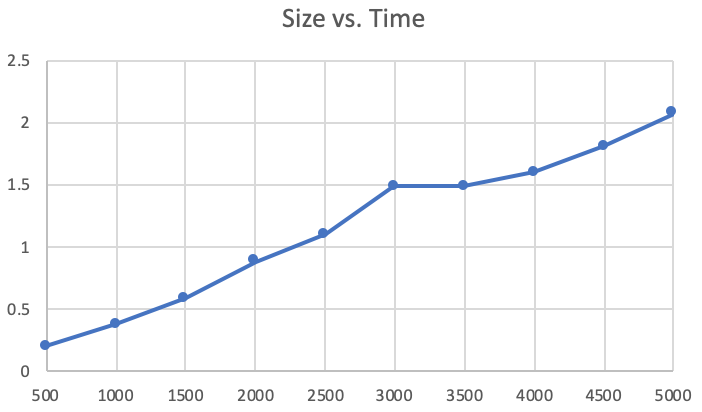
\includegraphics[height=6cm]{bayes_time_digit}
    \bigbreak
    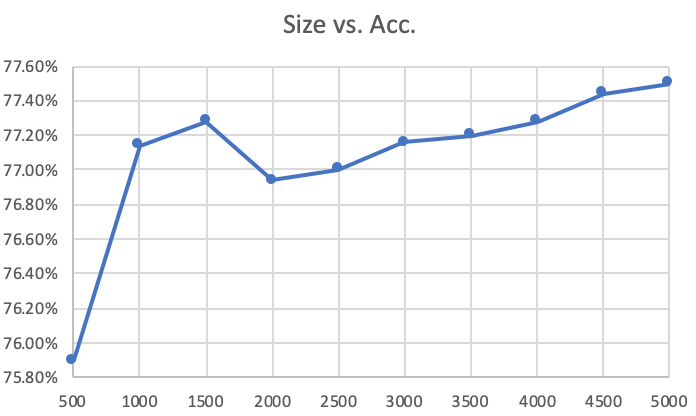
\includegraphics[height=6cm]{bayes_acc_digit}
    \bigbreak
    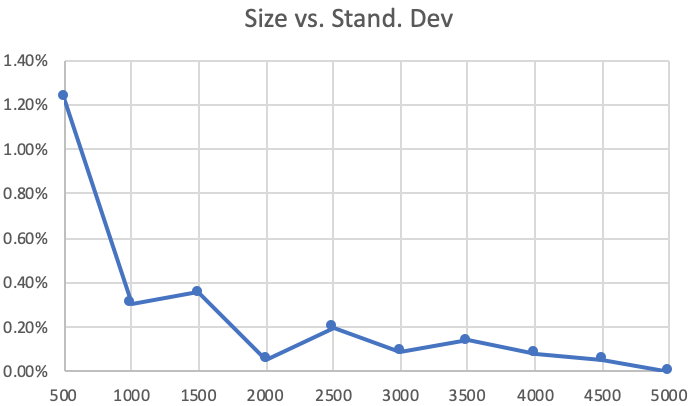
\includegraphics[height=6cm]{bayes_std_digit}

\pagebreak

\subsubsection{Face}
\begin{table}[h]
    \centering
    \resizebox{\textwidth}{!}{%
    \begin{tabular}{|l|l|l|l|}
    \hline
    \textbf{Training Size} & \textbf{Avg. Elapsed Time} & \textbf{Avg. Accuracy} & \textbf{Standard Deviation} \\ \hline
    45                     & 0.09304979 sec                & 80.40\%                & 8.28\%                      \\ \hline
    90                     & 0.16213244 sec                & 87.07\%                & 0.76\%                      \\ \hline
    135                    & 0.23094469 sec                & 88.53\%                & 0.56\%                      \\ \hline
    180                    & 0.29987997 sec                & 88.93\%                & 0.37\%                      \\ \hline
    225                    & 0.37142365 sec                & 89.60\%                & 0.89\%                      \\ \hline
    270                    & 0.44423203 sec                & 89.20\%                & 0.87\%                      \\ \hline
    315                    & 0.51784793 sec                & 88.13\%                & 0.56\%                      \\ \hline
    360                    & 0.58793861 sec                & 87.87\%                & 0.30\%                      \\ \hline
    405                    & 0.65206555 sec                & 88.40\%                & 0.37\%                      \\ \hline
    450                    & 0.7277254 sec                & 88.67\%                & 0.00\%                      \\ \hline
    \end{tabular}%
    }
    \end{table}
    \bigbreak
    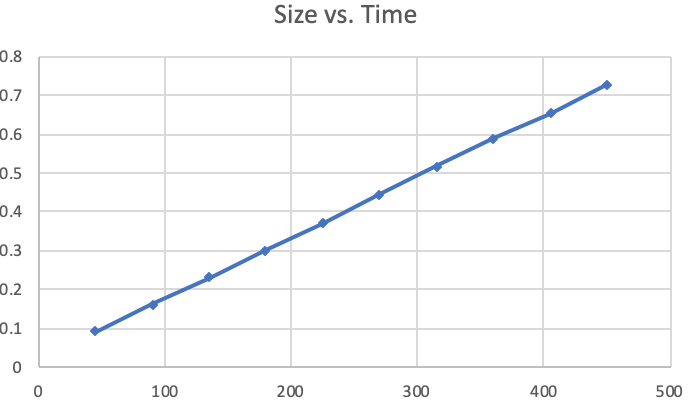
\includegraphics[height=6cm]{bayes_time_face}
    \bigbreak
    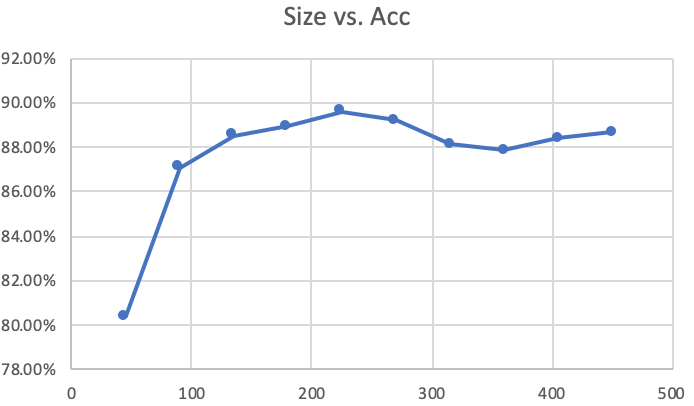
\includegraphics[height=6cm]{bayes_acc_face}
    \bigbreak
    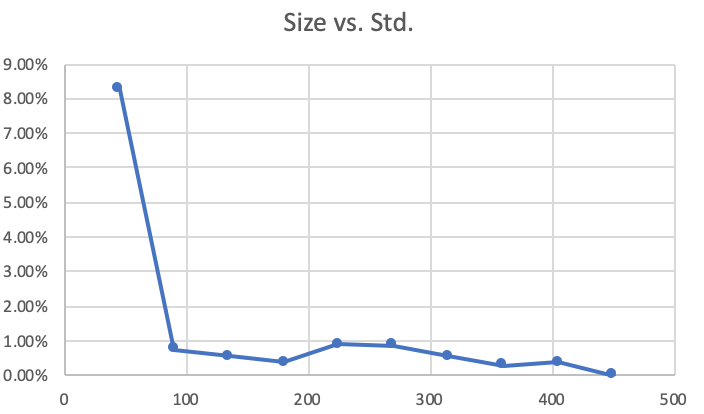
\includegraphics[height=6cm]{bayes_std_face}

\subsection{Perceptron}
\subsubsection{Digit}

\begin{table}[h!]
    \centering
    \resizebox{\textwidth}{!}{%
    \begin{tabular}{|l|l|l|l|}
    \hline
    \multicolumn{1}{|c|}{\textbf{Training Size}} & \multicolumn{1}{c|}{\textbf{Avg. Elapsed Time}} & \multicolumn{1}{c|}{\textbf{Avg. Accuracy}} & \multicolumn{1}{c|}{\textbf{Standard Deviation}} \\ \hline
    500                                          & 0.5149310443999997 sec                          & 70.12\%                                     & 7.245481350469408\%                              \\ \hline
    1000                                         & 0.9837744267999998 sec                          & 76.06\%                                     & 2.923696290656743\%                              \\ \hline
    1500                                         & 1.4807971413999979 sec                          & 77.9\%                                      & 2.3780243901188283\%                             \\ \hline
    2000                                         & 1.9622707825999952 sec                          & 78.98\%                                     & 1.4307340773183563\%                             \\ \hline
    2500                                         & 2.446689373399997 sec                           & 80.8\%                                      & 1.1895377253370303\%                             \\ \hline
    3000                                         & 2.966957307999999 sec                           & 79.52000000000001\%                         & 2.0092287077383704\%                             \\ \hline
    3500                                         & 3.4079184274 sec                                & 80.28\%                                     & 0.8318653737234125\%                             \\ \hline
    4000                                         & 3.8911088936 sec                                & 80.94\%                                     & 0.5458937625582442\%                             \\ \hline
    4500                                         & 4.367284299600004 sec                           & 79.12\%                                     & 2.0765355763867808\%                             \\ \hline
    5000                                         & 4.846412897199997 sec                           & 80.42\%                                     & 0.580517010947993\%                              \\ \hline
    \end{tabular}%
    }
    \end{table}
    \bigbreak
    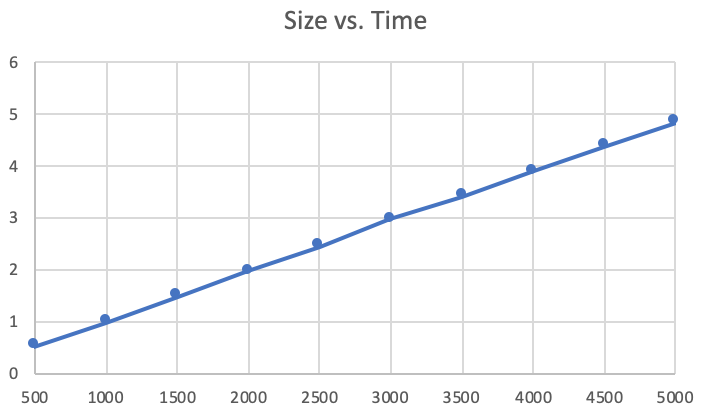
\includegraphics[height=6cm]{perc_time_digit}
    \bigbreak
    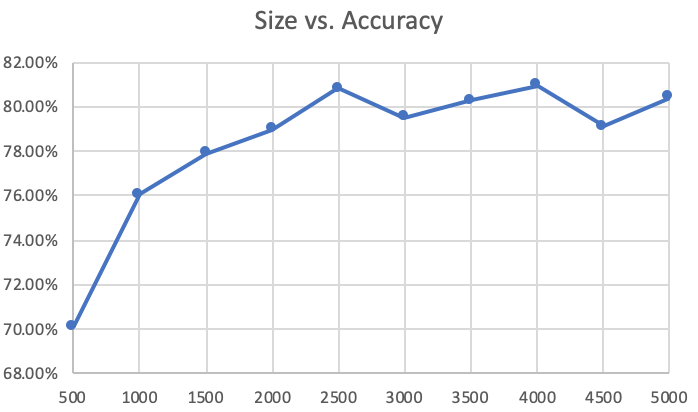
\includegraphics[height=6cm]{perc_acc_digit}
    \bigbreak
    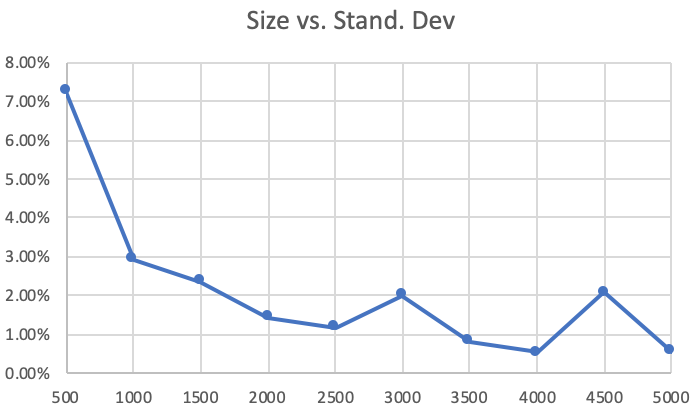
\includegraphics[height=6cm]{perc_std_digit}
\subsubsection{Face}
\begin{table}[]
    \centering
    \resizebox{\textwidth}{!}{%
    \begin{tabular}{|l|l|l|l|}
    \hline
    \textbf{Training Size} & \textbf{Avg. Elapsed Time} & \textbf{Avg. Accuracy} & \textbf{Standard Deviation} \\ \hline
    45                     & 0.08021645 sec                & 72.13\%                & 9.40\%                      \\ \hline
    90                     & 0.14196184 sec                & 82.67\%                & 5.91\%                      \\ \hline
    135                    & 0.20559907 sec                & 85.33\%                & 1.05\%                      \\ \hline
    180                    & 0.2708784 sec                 & 86.27\%                & 0.76\%                      \\ \hline
    225                    & 0.33621123 sec                & 85.87\%                & 0.30\%                      \\ \hline
    270                    & 0.41068009 sec                & 86.00\%                & 0.00\%                      \\ \hline
    315                    & 0.47430393 sec                & 86.00\%                & 0.00\%                      \\ \hline
    360                    & 0.53536463 sec                & 86.00\%                & 0.00\%                      \\ \hline
    405                    & 0.60785483 sec                & 86.00\%                & 0.00\%                      \\ \hline
    450                    & 0.67040364 sec                & 86.00\%                & 0.00\%                      \\ \hline
    \end{tabular}%
    }
    \end{table}
    \bigbreak
    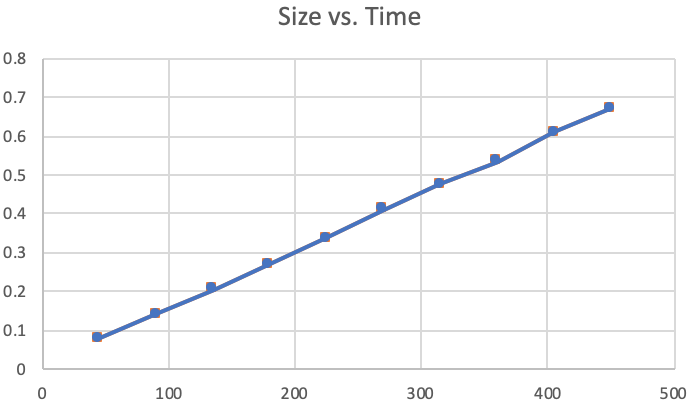
\includegraphics[height=6cm]{perc_time_face}
    \bigbreak
    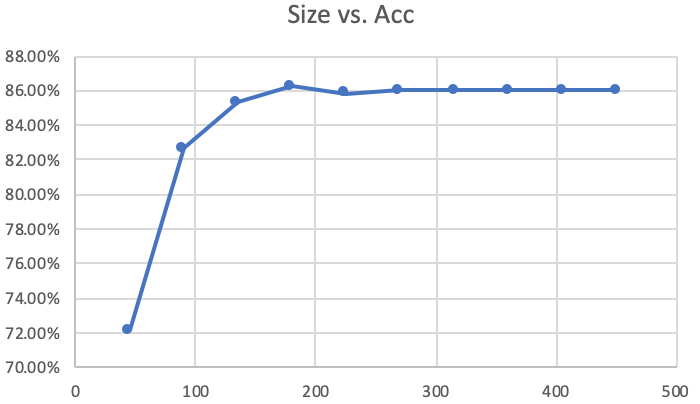
\includegraphics[height=6cm]{perc_acc_face}
    \bigbreak
    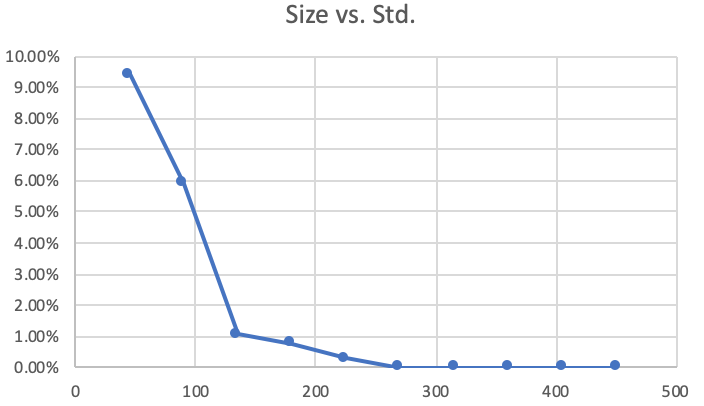
\includegraphics[height=6cm]{perc_std_face}
\subsection{Conclusion}

As expected, with an increase in training size came an increasing trend in accuracy and a decreasing trend in standard deviation. The more data there is to use to train the model means the testing will provide better and more consistent results. 
\\
\textbf{Digit:}
\begin{table}[h]
    \centering
    \resizebox{\textwidth}{!}{%
    \begin{tabular}{l|l|l|l|}
    \cline{2-4}
    \textbf{}                                 & \textbf{Avg. Elapsed Time} & \textbf{Avg. Accuracy} & \textbf{Standard Deviation} \\ \hline
    \multicolumn{1}{|l|}{\textbf{Bayes}}      & 2.0699248442000227 sec     & 77.5\%                 & 0.0\%                       \\ \hline
    \multicolumn{1}{|l|}{\textbf{Perceptron}} & 4.846412897199997 sec      & 80.42\%                & 0.580517010947993\%         \\ \hline
    \end{tabular}%
    }
    \end{table}
\\
\textbf{Face:}
\begin{table}[h]
    \centering
    \resizebox{\textwidth}{!}{%
    \begin{tabular}{l|l|l|l|}
    \cline{2-4}
    \textbf{}                                 & \textbf{Avg. Elapsed Time} & \textbf{Avg. Accuracy} & \textbf{Standard Deviation} \\ \hline
    \multicolumn{1}{|l|}{\textbf{Bayes}}      & 0.7277254 sec              & 88.67\%                & 0.00\%                      \\ \hline
    \multicolumn{1}{|l|}{\textbf{Perceptron}} & 0.67040364 sec             & 86.00\%                & 0.00\%                      \\ \hline
    \end{tabular}%
    }
    \end{table}

\noindent
For digit data, while Bayes was able to perform the training faster, it still had a lower accuracy than Perceptron. The Bayes model was able to reach a "plateu" of similar accuracy levels quicker than Perceptron tho, achieving relatively stable accuracy readings throughout the increase in sample size. 
For face data, Perceptron was able to perform the training quicker but had an overall less accurate performance. However, unlike for the digit data, the Perceptron model was able to reach a point of relative stability before the Bayes model. 


\end{document}
